% This is samplepaper.tex, a sample chapter demonstrating the
% LLNCS macro package for Springer Computer Science proceedings;
% Version 2.20 of 2017/10/04
%
\documentclass[runningheads]{llncs}
%
\usepackage{graphicx}
% Used for displaying a sample figure. If possible, figure files should
% be included in EPS format.
%
% If you use the hyperref package, please uncomment the following line
% to display URLs in blue roman font according to Springer's eBook style:
% \renewcommand\UrlFont{\color{blue}\rmfamily}

\usepackage{amsmath}
\usepackage{amsfonts}
\usepackage{graphicx}
\usepackage{diagbox}
\usepackage{multirow}
\usepackage{booktabs}
\usepackage{float}
\usepackage{url}
\usepackage{float}
\usepackage[linesnumbered, boxed, ruled]{algorithm2e}

\usepackage[all]{xy}
\usepackage{setspace}

\usepackage{geometry}
\usepackage{caption}
\captionsetup[table]{skip=5pt}
%\geometry{left=2.0cm, right=2.0cm, top=2.5cm, bottom=2.5cm}

%\setlength{\abovecaptionskip}{0pt}
%\setlength{\belowcaptionskip}{0pt}

\newcommand{\tabincell}[2]{\begin{tabular}{@{}#1@{}}#2\end{tabular}}

\begin{document}
	
\renewcommand\arraystretch{1.5}

%
\title{Aligning Sentences between Comparable Texts \\of Different Styles}
%
%\titlerunning{Abbreviated paper title}
% If the paper title is too long for the running head, you can set
% an abbreviated paper title here
%
\author{Xiwen Chen \and Mengxue Zhang \and Kenny Q. Zhu}
%
\authorrunning{Chen et al.}
% First names are abbreviated in the running head.
% If there are more than two authors, 'et al.' is used.
%
\institute{Advanced Data and Programming Technology Lab \\
	Computer Science Dept. \\
	Shanghai Jiao Tong University, 800 Dong Chuan Rd. \\
	\url{https://adapt.seiee.sjtu.edu.cn/}\\
	\email{\{victoria-x@sjtu, lovealice@sjtu, kzhu@cs.sjtu\}.edu.cn}}

\maketitle              % typeset the header of the contribution
%
\begin{abstract}
Monolingual parallel corpus is crucial for training and evaluating text rewriting or paraphrasing models. Aligning parallel sentences between two large body of texts is a key step toward automatic construction of such parallel corpora. We propose a greedy alignment algorithm that makes use of strong unsupervised similarity measures. The algorithm aligns sentences with state-of-the-art accuracy while being more robust on corpora with special linguistic features. Using this alignment algorithm,  we automatically constructed a large English parallel corpus from various translated works of classic literature.

\keywords{Monolingual parallel corpora  \and Sentence alignment \and Unsupervised algorithms.}
\end{abstract}
%
%
%
\begin{spacing}{1.1}
\section{Introduction}
\label{sec:intro}

In natural language processing, there are many supervised learning models that require the existence of parallel corpus for training. However, manual annotation, which is used in constructing many reliable parallel corpora, is inefficient and time-consuming. Cross-lingual sentence alignment has been extensively studied for machine translation, but the construction of monolingual parallel corpus is also gaining its interest. For cross-lingual alignment, different words are relatively discriminative in data distribution, while in monolingual alignment, the ``style'' of a word might be much more subtle to distinguish. Monolingual parallel corpora can be used to learn text rewriting rules, which is involved in sentence simplification, natural language style transfer, and document summarization~\cite{hwang2015aligning}. It can also be used to learn the relation between monolingual texts such as semantic relatedness and similarity.

The monolingual sentence alignment model takes two comparable monolingual texts as an input, and outputs a $x$-to-$y$ alignment of these two corpora, where the sequential combination of $x$ sentences from the first corpus is aligned with $y$ sentences from the second corpus, and both combinations are ``similar'' in content. For instance, the following sentences, although different in their expressions, can be properly aligned to each other in terms of content.

\emph{Alyosha got up, walked over to the door, and reported that no one was listening to them.}

\emph{Alyosha went, opened the door a little, and reported that no one was eavesdropping.}

In previous research, mainly one-to-one and $n$-to-one matching schemes are studied. When only one-to-one sentence mapping is assumed, the similarity scores for each pair of sentences can be precomputed~\cite{kajiwara2016building}, which largely simplifies the problem. However, this condition does not hold for literature corpora, since one sentence might be rephrased as different number of sentences in another expression. In the work of Hwang et al.~\cite{hwang2015aligning}, many-to-one mappings are taken into consideration to align simple and standard Wikipedia, which is a safe assumption because a sentence in standard Wikipedia is very likely to be broken into several short sentences in simple Wikipedia. But this is not the case for general comparable texts. Our $x$-to-$y$ sentence mapping assumption is more challenging but practical.

The challenge of our problem is two-fold. First, similarity measure of sentences, which is crucial in alignment decision, is difficult to design for different corpora with different semantic features. Second, in each aligned pair, the number of successive sentences on each side is not known in advance but has to be discovered during the sequential alignment process. Moreover, some measurements that show higher accuracy in similarity evaluation work relatively slow when aligning large corpora. Therefore, the similarity measure for every possible pair and every possible sentence length cannot be assumed to be known, and thus the problem cannot be resolved as a simple matching problem. The second challenge is more significant in our $x$-to-$y$ matching scheme. These challenges are not present in previous problems, but are inevitable in our case because the monolingual documents differ in ``style'' in general and not as specific as ``simple/complex''.

The contributions of this work are the following.
\begin{enumerate}
	\item We extend the monolingual alignment problem to the $x$-to-$y$ matching solution of two documents in different styles, and devise an unsupervised alignment scheme that produces high-quality matching pairs. The styles of documents are not limited to simple/complex language (Section \ref{sec:method}).
	\item We experiment similarity measures based on Word2Vec model~\cite{mikolov2013distributed}, Universal Sentence Encoder~\cite{cer2018universal} and InferSent model~\cite{conneau2017supervised}. We evaluate the performance of these measures and compare with baseline models for paraphrase detection, and verify that our unsupervised methods have comparable performances with state-of-art (supervised and unsupervised) methods (Section \ref{sec:results}).
	\item Using a greedy algorithm and a filter mechanism for sequence alignment, we compare the performances of our model with baseline sentence alignment models on literature works with different linguistic characteristics. The results show that the filter mechanism can significantly improve the quantity of aligned sentences while preserving a reasonable quality (Section \ref{sec:method} and \ref{sec:results}).
	\item We construct a monolingual parallel corpus from various literature translations. This corpus can be used to learn general text rewriting models, and specifically, the ``style'' of a text (Section \ref{sec:data}).
\end{enumerate}

% ==============================================================================================================

\section{Related Work}
\label{sec:related}

With several exceptions, the sentence similarity measure task is fulfilled in two general approaches: (a) sentence embeddings or word embeddings are first obtained and similarity score is calculated based on mathematical measure on vector distance, such as normalized Euclidean distance, cosine distance and earth mover's distance, or (b) similarity score is learned by semantic features or distributional statistics.

In explorations of word-level similarities, word vectors mostly relied on pretrained word vectors such as GloVe~\cite{pennington2014glove} and fasttext~\cite{joulin2017bag} pretrained word vectors. Then word-level similarity and multiple word alignment rules are applied to obtain sentence-level similarities. By directly obtaining sentence vectors, other studies focused more on the forms of distance measure for sentence vectors to better capture the real semantic distance~\cite{kajiwara2016building}.

Based on word embeddings, Zhu et al. constructed a parallel corpus for text simplification using cosine similarity between TF-IDF vectors of sentences~\cite{zhu2010monolingual}. Later studies considered more sentence semantic features including sentence ordering~\cite{coster2011learning} and word-level similarity~\cite{hwang2015aligning}. Kajiwara et al. used four word-level alignment methods for similarity measure, and constructed a monolingual parallel corpus for text simplification using similarity matrix and a given threshold~\cite{kajiwara2016building}. Hatzlvassiloglou et al. evaluated the incorporation of multiple linguistic features and the combinations of them in text similarity measure~\cite{hatzlvassiloglou1999detecting}.

In sentence alignment task, Zamani et al. modeled the sequential alignment process using integer programming, arguing that a weak similarity measure is compensated by an optimal sequential alignment algorithm~\cite{zamani2016sentence}. Hwang et al. compared a greedy alignment pattern with an ordered alignment algorithm by dynamic programming, and proved the practical priority of the former~\cite{hwang2015aligning}.

% ==============================================================================================================


\section{Methodology}
\label{sec:method}

An overview of the model architecture is shown in Figure \ref{fig:4}. Under the assumption that the two documents have comparable order in sentences, the model aligns the two texts as follows.
\begin{enumerate}
	\item Given a similarity measure $f_1$, the similarity measurement model computes the scores for all possible one-to-one pairs within a certain distance. This distance is defined as \texttt{MAX\_DISTANCE}, and is the maximum relative distance (given by the index of a sentence in the document) between two single sentences that are considered at this stage.
	\item Pairs whose similarity scores are above a given threshold $t$ are supposed to be the ``anchors'' and are appended to an anchor list. The anchors divide the original document into parts that are relatively shorter and easier for later alignment.
	\item For each part between two pairs of anchors, a local alignment algorithm is performed using a certain similarity measure, where we need to group the sentences and then align the groups.
	\item Finally, an optional filtering process is performed. This is due to the observation that, including only one kind of similarity measure might result in unreasonable alignment or too strict alignment rules. To capture the semantic features in different perspectives, an additional similarity measure can be used to perform a filtering stage for sentences that are not successfully aligned at previous stages. At this stage, we only consider one-to-one alignment.
\end{enumerate}

\begin{figure}[htbp]
	\centering
	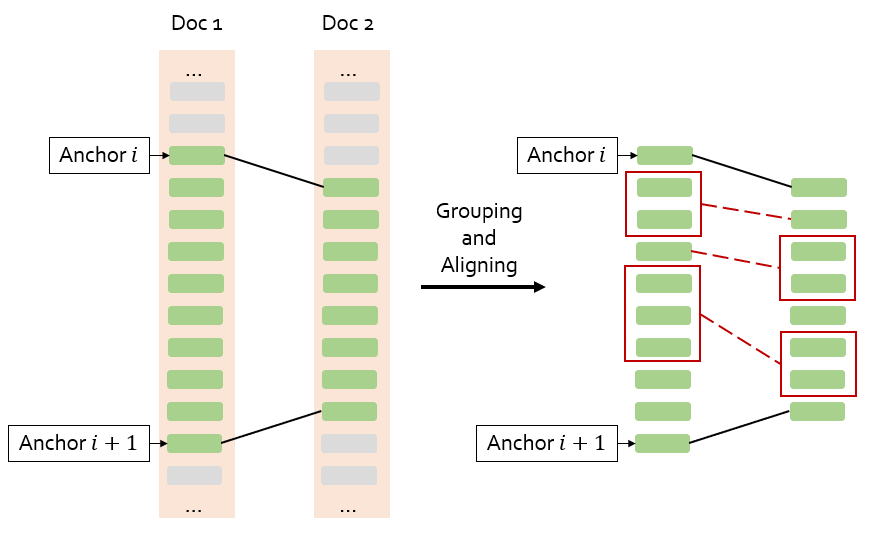
\includegraphics[width=12cm]{./4.PNG}
	\caption{Model Overview.}\label{fig:4}
\end{figure}

In sum, the model consists of basic similarity measurements and a local sequential alignment in each part separated by successive anchors. The effect of the final filtering stage will also be explored in this work.


\subsection{Similarity Measure}

The first subtask is to give a similarity score for each pair of sentences in order to further align them. In practice, the scoring requires a clustering strategy, since one-to-one sentence mapping is not necessarily required in the sequential alignment task. At this stage, we restrict ourselves to first evaluating the performance of different similarity measures. Namely, given two sentences $(w_1^{(a)}, w_2^{(a)}, \ldots, w_{l_a}^{(a)})$ and $(w_1^{(b)}, w_2^{(b)}, \ldots, w_{l_b}^{(b)})$, where each word in the sequence is a fixed dimensional vector $w_i^{(a)}, w_j^{(b)}\in \mathbb{R}^d$. Then each pair of the sentences $a, b$ are mapped to a score $r\in [0, 1]$ representing their sentence similarity. The compared models are evaluated based on their accuracies of paraphrase detection task, with corpora including MSRC, SICK, and Shakespeare scripts.

The general approach for unsupervised similarity measure is composed of a (hopefully strong) sentence representation model and a simple distance measure.
\begin{itemize}
	\item \textbf{Gensim Word2Vec (WDV).} The Gensim implementation of Word2Vec model uses CBOW and Skip-gram models~\cite{mikolov2013distributed}. In our implementation, the word vectors are trained on the two documents to be aligned, rather than using pretrained word vectors given by independent large corpus. This is under the consideration that, since our sentence alignment task is performed on stylized sentences, a corpus-specific Word2Vec model better fits in our scheme.
	
	After obtaining word embeddings, the sentence embedding is the average of the sum of word vectors in a sentence. Then the final similarity is the average of word similarities according to a max alignment. Each word in sentence 1 is aligned to the most similar word in sentence 2, while each word in sentence 2 is aligned to the most similar word in sentence 1. Then the scores for the alignments in both directions are added and normalized by sentence length.
	\item \textbf{Universal Sentence Encoder (UNV).} Universal Sentence Encoder proposed by Cer et al.~\cite{cer2018universal} is designed to encode sentences into embedding vectors that specifically target transfer learning. This model is found to be useful in the filtering stage in this study.
	\item \textbf{InferSent Model (INF).} InferSent model first proposed as a Facebook research project of learning universal representations of sentences~\cite{conneau2017supervised}. In our study, we explore both GloVe and FastText pretrained word vectors proposed in their model~\cite{pennington2014glove, joulin2017bag}.
\end{itemize}

Using sentence embeddings, cosine and arccos measures are used to calculate the final similarity score, defined as follows.
\begin{align*}
sim_{\cos} & = \cos(v_1, v_2), \\
sim_{\arccos} & = 1 - \frac{\arccos(\cos(v_1, v_2))}{\pi}.
\end{align*}
Particularly, it is shown from the results that cosine distance measure is superior to the arccos measure.

These unsupervised methods are compared with the state-of-art supervised methods in paraphrase detection task, in order to evaluate the ability of the similarity measures used in the alignment. These methods include:
\begin{itemize}
	\item Siamese Recurrent Neural Networks (MaLSTM)~\cite{mueller2016siamese}.
	\item TF-KLD: a discriminative improvement to distributional sentence similarity proposed by Ji et al.~\cite{ji2013discriminative}.
\end{itemize}

\subsection{Sequential Alignment}

In our scheme of constructing parallel corpus from comparable documents, we need to consider (a) the documents being aligned are potentially large, and (b) there exist sentences that are aligned with two or more sentences from the other document, and there also exist sentences that are not aligned at all.

These two scenarios lead to challenges in designing the sequential alignment algorithm, since the grouping of the sentences are not known in advance, the similarity score for each pair of groups is not pre-calculated. Furthermore, exhaustive enumeration of all possible groupings is intractable. Therefore, we make the following assumptions.
\begin{enumerate}
	\item The number of sentences in each group does not exceed a maximum window size \texttt{MAX\_WINDOW\_SIZE} for each part enclosed by any two successive anchors of the document. Moreover, to handle the situation of shorter parts, the maximum number of sentences is proportional to a factor, defined as \texttt{SIZE\_PER\_TEN}. The scaled limit
	$$w_{max} = \texttt{SIZE\_PER\_TEN} \times \texttt{len}(part) / 10$$
	is then compared with \texttt{MAX\_WINDOW\_SIZE}, and the minimum of them is the maximum number of sentences in a group.
	\item Two aligned groups cannot appear farther than a limit \texttt{MAX\_DISTANCE}. The assumption is that the aligned groups in the two documents do not locate far from each other, considering relative distance for the whole document. Suppose the index of a sentence in \emph{doc1} is $i$, then the relative corresponding index in \emph{doc2} is defined by $j = i\cdot \dfrac{l_2}{l_1}$, where $l_k, k = 1, 2$ denotes the document length, and the sentences in \emph{doc2} out of the range [$j$ - \texttt{MAX\_LENGTH}, $j$ + \texttt{MAX\_LENGTH}] will not be considered.
\end{enumerate}

Based on these assumptions, we use a greedy alignment scheme. Between each successive pairs of anchors, the similarity scores for all possible pairs are calculated and sorted in decreasing order. In each pairing, the most similar pair is popped from the candidate list, and the remaining groups that include any sentence in the selected pair is deleted from the candidate list. The pairing stops until the similarity score for the most similar pair is below a predefined threshold, or the candidate list becomes empty. The greedy alignment process is illustrated in Algorithm \ref{alg:1}.

\begin{algorithm}
	\caption{Greedy Alignment.}
	\label{alg:1}
	\KwIn{A sorted array (based on similarity score $sim$) of sentence group pairs $Arr = [[g_1, g_2, sim], \ldots]$}
	\KwOut{An collection of paired sentence groups}
	$A\leftarrow \emptyset$\;
	\While{$Arr[0].sim > threshold$}{
		$p\leftarrow Arr.pop(0)$\;
		Add $p$ into $A$;
		\ForEach{sentence $s$ in $p.g_1$}{
			remove $p'$ from $Arr$ if $p'.g_1$ contains $s$\;
		}
		\ForEach{sentence $s$ in $p.g_2$}{
			remove $p'$ from $Arr$ if $p'.g_2$ contains $s$\;
		}
	}
	\textbf{return} $A$\;
\end{algorithm}

% ==============================================================================================================

\section{Experimental Setup}
\label{sec:exp}

We design two experiments, one for evaluating different similarity measures, and the other one for the sentence alignment. The datasets and metrics used are introduced below.

\subsection{Similarity Measure}

The similarity measure is evaluated based on a paraphrase detection task performed on Microsoft Research Paraphrase Corpus (MSRC), SICK, and Modern/Original Version of Shakespeare scripts. For unsupervised similarity measure, the three sentence embedding schemes with multiple embedding dimensions for word embeddings are combined with the two distance measures, and together with a set of thresholds, are used to label sentences with a similarity score above threshold as paraphrases. We also used BLEU~\cite{papineni2002bleu} and ROUGE~\cite{lin2004rouge}, as baseline models in this task.

\subsection{Sentence Alignment}

The datasets on sentence alignment are a part of the final documents that are aligned, including \emph{Anna Karenina}, \emph{The Story of Stone} and \emph{The Brothers Karamazov}. Related data for each corpus is shown in Table \ref{tb:1}.

\begin{table}[h!]\footnotesize
	\centering
	\small
	\begin{tabular}{|c|c|c|}
		\hline
		Corpus & Translation 1 & Translation 2 \\
		\hline
		Anna Karenina & 21,398 & 20,973 \\
		The Story of Stone & 46,034 & 56,256 \\
		The Brothers Karamazov & 24,133 & 20,288 \\
		\hline
	\end{tabular}
	\caption{Size of Datasets (Number of Words).}\label{tb:1}
\end{table}

The evaluation of sentence alignment is based on the following considerations.
\begin{enumerate}
	\item \emph{Efficiency.} The time a model takes to align sentences should be reasonable with respect to the number of sentences in the raw documents.
	\item \emph{Percentage of aligned sentences.} Although the main focus of this research is to construct a corpus with high quality, the percentage of aligned sentences should also be considered. Namely, we want to assess how many sentences should be aligned are actually aligned by the model.
	\item \emph{Quality.} Since it is hard to assess whether all sentences are properly aligned or not, we sample a fraction of aligned sentences and decide whether each pair should be aligned manually. The quality of the alignment is evaluated as the percentage of the pairs that are ``properly aligned'' with respect to the number of total aligned pairs. The level of properness for a aligned pair is defined as follows, based on Huang's criteria~\cite{hwang2015aligning}.
	\begin{itemize}
		\item \textbf{Good}:
		\begin{enumerate}
			\item completely the same;
			\item possibly some word substitutions and structural modifications;
			\item describe the same object, environment, or situation using different but the same type of adjectives, nouns, sentiments, etc.;
			\item convey the same type of sentiments in short conversations.
		\end{enumerate}
		\item \textbf{Good Partial}:
		\begin{enumerate}
			\item one sentence is good aligned with respect to a part of the other sentence;
			\item the sentence contains some additional clauses or phrases that have information which is not contained within the other sentence;
		\end{enumerate}
		\item \textbf{Partial}:
		\begin{enumerate}
			\item a part of a sentence is good aligned with respect to a part of the other sentence;
			\item both sentences contain some additional clauses or phrases that have information which is not contained within the other;
		\end{enumerate}
		\item \textbf{Bad}: the sentences discuss unrelated contents.
	\end{itemize}
	From above, the first three categories are considered as ``properly aligned''. The definition is relatively loose for stylized expressions. It happens that in an aligned sentence pair, one contains additional expressions than the other. But the main content of the pair should be consistent.
\end{enumerate}

For the following discussion, the ``percentage'' represents the portion of sentences that are aligned in the raw documents, and the ``quality'' represents the portion of aligned pairs that are proper.

\section{Results}
\label{sec:results}

Experimental results for similarity measure and sentence alignment are presented in the next two sections. It is shown that the unsupervised similarity measure is comparable with supervised similarity measures, and that we have a relatively strong similarity scoring system for sentence alignment. Then we verify that our sentence alignment model is superior to the baseline model in terms of robustness and quality.

\subsection{Similarity Measure}
The result for MSRC with different thresholds is shown in Figure \ref{fig:5}. From the figure we can observe that the highest accuracy is reached by ``WDV + MAX + COS'' at threshold around 0.7, with the second highest accuracy reached by the ``UNV + COS'' combination.

\begin{figure}[htbp]
	\centering
	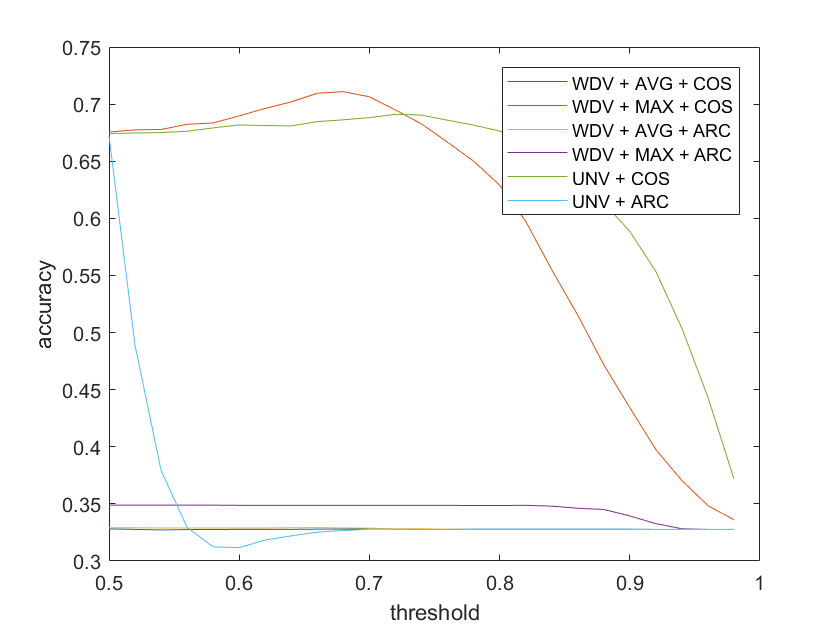
\includegraphics[width=8cm]{./5.png}
	\caption{Accuracies for MSRC with Different Threshold $t$.}\label{fig:5}
\end{figure}

One observation is that the cosine measurement is superior to the arccos measurement, which is the case also for SICK and Shakespeare (SHPR). This might be an indication that cosine measure is a more reasonable measure for spatial distance in the vector space of sentence embeddings.

For each experimented similarity measurement method, the best dimension for word embedding and the best threshold is used for the final comparison. The dimension is fixed as 100. The results for both supervised and unsupervised methods are shown in Table \ref{tb:2}. (INF-F and INF-G are InferSent models using GloVe and fasttext pretrained word vectors, respectively.)

\begin{table}[h!]\footnotesize
	\centering
	\small
	\begin{tabular}{|c|c|c|c|}
		\hline
		\diagbox{Method}{Accuracy (\%)}{Corpus} & MSRC & SICK & SHPR \\
		\hline
		\hline
		WDV + AVG + COS & 32.8 & 36.6 & 52.5 \\
		WDV + MAX + COS & 71.1 & 68.1 & 72.0 \\
		WDV + AVG + ARC & 32.9 & 36.7 & 53.9 \\
		WDV + MAX + ARC & 34.9 & 39.4 & 54.7 \\
		UNV + COS & 67.9 & \textbf{74.2} & 77.6 \\
		UNV + ARC & 67.2 & 63.5 & 50.0 \\
		INF-F + COS & \textbf{72.2} & 72.5 & \textbf{78.6} \\
		INF-F + ARC & 67.2 & 63.5 & 50.6 \\
		INF-G + COS & 70.4 & 73.0 & 73.9 \\
		INF-G + ARC & 67.2 & 63.4 & 50.8 \\
		\hline
		MaLSTM & 56.9 & 78.3 & 71.6 \\
		TF-KLD & 70.8 & 74.5 & 86.1 \\
		\hline
		BLEU & 69.9 & 65.9 & 71.0 \\
		ROUGE & 71.3 & 67.8 & 71.8 \\
		\hline
	\end{tabular}
	\caption{Paraphrase Detection Accuracies.}\label{tb:2}
\end{table}

From the results, we can conclude that the similarity measurement ability on both standard paraphrase corpus and literature corpus is competent compared with state-of-art similarity models, and especially, supervised models. In the sentence alignment task, the ability to measure sentence similarity and the efficiency of this evaluation should both be considered, since the documents to be aligned might be so large that the sentence encoding model costs a lot of computing resources.

\subsection{Sentence Alignment}

Table \ref{tb:7} shows how filter mechanism affects the alignment quantity and quality\footnote{The model names are abbreviated as ``model + filter'' schemes. For instance, ``BLEU + UNV'' means BLEU model for the first three stages of alignment, and Universal Sentence Encoder model for the last stage of filtering.}. The results verify that our filter scheme does largely improve the overall performances of alignment models. Specifically, ``BLEU + UNV'' and ``WDV + UNV'' combinations outperform other models in both quality and quantity, these two combinations will be used for end-to-end comparison.

\begin{table*}[htbp]\footnotesize
	\centering
	\small
	\begin{tabular}{|c|c|c|c|c|c|c|c|c|c|c|}
		\hline
		\textbf{\diagbox{Result}{Model}} & \textbf{BLEU} & \textbf{INF} & \textbf{WDV} & \textbf{UNV} & \textbf{\tabincell{c}{BLEU \\ + \\ UNV}} & \textbf{\tabincell{c}{BLEU \\ + \\ INF}} & \textbf{\tabincell{c}{WDV \\+ \\ UNV }} & \textbf{\tabincell{c}{WDV \\ + \\ INF }} & \textbf{\tabincell{c}{INF \\ + \\ UNV }} & \textbf{\tabincell{c}{UNV \\ + \\ INF }}  \\
		\hline
		\hline
		Time & 1.9m & 8.4m & 4.5m & 1.7h & 10.8m & 9.8m & 19.4m & 8.1m & 24.8m & 3.6h \\
		Percentage [\%] & 73.7 & 70.9 & 73.7 & 42.2 & 87.1 & 85.0 & 85.6 & 85.2 & 17.7 & 53.6  \\
		Quality [\%] & 100 & 98 & 98 & 91 & 100 & 100 & 98 & 97 & 100 & 99 \\
		\hline
	\end{tabular}
	\caption{Quantitative Results (\emph{Notre Dame de Paris}).}\label{tb:7}
\end{table*}

We perform our alignment model on other three pairs of documents, \emph{Anna Karenina}, \emph{The Story of Stone}, and \emph{The Brothers Karamazov}. The results are shown in Table \ref{tb:8}.

\begin{table*}[htbp]\footnotesize
	\centering
	\small
	\begin{tabular}{|c|c|c|c|c|c|c|c|}
		\hline
		\textbf{\diagbox{Model}{Result}} & Time & Percentage [\%] & G [\%] & GP [\%] & P [\%] & B [\%] & Quality [\%] \\
		\hline
		\multicolumn{8}{|c|}{Anna Karenina} \\
		\hline
		This work & 0.78h & \textbf{68.7} & 90 & 5 & 3 & 2 & \textbf{98} \\
		Bleualign & 23.44s & 37.2 & 53 & 19 & 5 & 23 & 77 \\
		\hline
		\multicolumn{8}{|c|}{The Story of Stone} \\
		\hline
		This work & 8.2h & 19.2 & 35 & 29 & 16 & 20 & \textbf{80} \\
		Bleualign & 51.56s & 25.5 & 10 & 11 & 19 & 60 & 40 \\
		\hline
		\multicolumn{8}{|c|}{The Brothers Karamazov} \\
		\hline
		This work & 1.1h & \textbf{53.2} & 67 & 24 & 7 & 2 & \textbf{98} \\
		Bleualign & 24.33s & 33.0 & 32 & 38 & 9 & 21 & 79 \\
		\hline
	\end{tabular}
	\caption{Quantitative Results ([1] \emph{Notre Dame de Paris}, [2] \emph{The Story of Stone}) G: Good, GP: Good Partial, P: Partial, B: Bad.}\label{tb:8}
\end{table*}

Although the baseline model, Bleualign performs the fastest among the compared schemes, it does not guarantee the quality of aligned sentences. Moreover, since it highly relies on word alignment, it fails in aligning comparable documents that are not so much alike at the first glance, such as \emph{The Story of Stone}. The following shows a sample pair which is misaligned by the Bleualign model, but is properly aligned by our method.

\textbf{Sentence}: \emph{His second child was a daughter, born strangely enough on the first day of the year.}

\textbf{Bleualign}: \emph{The first qin emperor,}

\textbf{Our model}: \emph{The second child she bore him was a little girl, rather remarkable because she was born on new year day.}

As a qualitative analysis on model misbehaviors, we take a few representative sentences from the results that are not properly aligned by different models in the experiment, as is in Table \ref{tb:4}.

One can notice that word-based alignment schemes, such as BLEU, WDV, and the Bleualign model, is not competent in handling short sentences, while sentence-based alignment schemes fail in cases of longer sentences. This can serve as an argument for using similarity measurements from both perspectives, as a compensation for each other. Furthermore, word-level similarity measures can serve as better anchors in the first stage of our model, and sentence-level similarity measures serve well as filters in the second stage, since sentence level encoders normally takes longer time to embed sentences in every single run.

\begin{table*}[h!]\footnotesize
	\centering
	\small
	\begin{tabular}{|c|c|}
		\hline
		\textbf{Model} & \textbf{Misaligned Sentence (False Positive [FP] or False Negative [FN])}  \\
		\hline
		\hline
		Bleualign [FP] & \tabincell{c}{\emph{baoyu clapped his hands in approval.} \\ \emph{you're getting quite a temper lately, master bao.}}  \\
		\hline
		BLEU [FN] & \tabincell{c}{\emph{xiang-yan and bao-chai were present that day, it was true; but the absence of...to burst into tears.} \\ \emph{seeing xiangyun and baochai there but not...wanted to take off some clothes.}}  \\
		\hline
		INF [FP] & \tabincell{c}{\emph{the priest whom the girls had noticed...was indeed archdeacon claude frollo.} (31 words) \\ \emph{but she has three things...hands by squeezing her waist.} (79 words)}  \\
		\hline
		WDV [FP] & \tabincell{c}{\emph{what's at stake here are the women.} \\ \emph{are there women or are there not?}} \\
		\hline
		UNV [FP] & \tabincell{c}{\emph{the mob repeated with a frenzied cheer.} \\ \emph{and among the monsters thus...in front of a candle.} (48 words)}  \\
		\hline
	\end{tabular}
	\caption{Aligned Corpora.}\label{tb:4}
\end{table*}

\section{Constructing a Monolingual Parallel Corpus}\label{sec:data}

We then proceed to construct a monolingual parallel corpus using the sentence alignment model. The corpus mainly comes from different versions of translation of 10 literature works. A complete list of information about the aligned works is shown Table \ref{tb:6}.

To evaluate the quality of the alignment, a sample batch of sentences are selected and manually decided on whether the alignment is reasonable based on the criteria described above. The quality of the parallel corpus is represented by the percentage of ``true positive'' with respect to the total number of aligned pairs. Our work achieves reasonable alignment efficiency and generates high quality sentences for text rewriting rules.

\begin{table*}[h!]\footnotesize
	\centering
	\small
	\begin{tabular}{|c|c|c|c|c|c|}
		\hline
		\textbf{\diagbox{Corpus}{Information}} & \textbf{Author} & \textbf{Translator} & \textbf{Length} & \textbf{Aligned (\%)} & \textbf{Quality (\%)} \\
		\hline
		\hline
		\multirow{2}{*}{Notre Dame de Paris} & \multirow{2}{*}{Victor Hugo} & Alban Krailsheimer & 10272 & 86.3 & \multirow{2}{*}{99.4} \\
		\cline{3-5}
		& & I. F. Hapgood & 10179 & 87.0 & \\
		\hline
		\multirow{2}{*}{Les Miserables} & \multirow{2}{*}{Victor Hugo} & Julie Rose & 34145 & 76.4 & \multirow{2}{*}{99.0} \\
		\cline{3-5}
		& & I. F. Hapgood & 34328 & 76.0 & \\
		\hline
		\multirow{2}{*}{The Story of Stone} & \multirow{2}{*}{Cao Xueqin} & Yang Xianyi & 46034 & 9.7 & \multirow{2}{*}{94.0} \\
		\cline{3-5}
		& & David Hawkes & 56256 & 8.6 &  \\
		\hline
		\multirow{2}{*}{The Brothers Karamazov} & \multirow{2}{*}{F. Dostoevsky} & A. R. MacAndrew & 24133 & 58.6 & \multirow{2}{*}{95.3} \\
		\cline{3-5}
		& & Richard Pevear & 20288 & 68.1 & \\
		\hline
		\multirow{2}{*}{Crime and Punishment} & \multirow{2}{*}{F. Dostoevsky} & Michael R. Katz & 14503 & 70.6 & \multirow{2}{*}{93.9} \\
		\cline{3-5}
		& & Richard Pevear & 12938 & 76.2 & \\
		\hline
		\multirow{2}{*}{The Magic Mountain} & \multirow{2}{*}{Thomas Mann} & John E. Woods & 14464 & 83.8 & \multirow{2}{*}{97.6} \\
		\cline{3-5}
		& & H. T. Lowe-Porter & 14231 & 83.8 & \\
		\hline
		\multirow{2}{*}{The Illiad} & \multirow{2}{*}{Homer} & Ian C. Johnston & 7744 & 68.1 & \multirow{2}{*}{72.5} \\
		\cline{3-5}
		& & Robert Fagles & 7237 & 58.5 & \\
		\hline
		\multirow{2}{*}{Don Quixote} & \multirow{2}{*}{Cervantes Saavedra} & John Rutherford & 11902 & 48.5 & \multirow{2}{*}{84.4} \\
		\cline{3-5}
		& & John Ormsby & 9056 & 58.3 & \\
		\hline
		\multirow{2}{*}{Anna Karenina} & \multirow{2}{*}{Leo Tolstoy} & Pevear and Volokhonsky & 21398 & 74.6 & \multirow{2}{*}{99.3} \\
		\cline{3-5}
		& & Rosamund Bartlett & 20971 & 74.5 & \\
		\hline
		\multirow{2}{*}{Madame Bovary} & \multirow{2}{*}{Gustave Flaubert} & Eleanor Marx-Aveling & 6670 & 73.9 & \multirow{2}{*}{97.6} \\
		\cline{3-5}
		& & Margaret Mauldon & 6837 & 72.8 & \\
		\hline
	\end{tabular}
	\caption{Aligned Corpora.}\label{tb:6}
\end{table*}

In order to guarantee the quality of the corpus, the percentage of aligned sentences with respect to the original length is not necessarily maximized. Besides, some aligned pairs contain sentences that are exactly identical. We did not discard them, since in order to learn monolingual text rewriting rules, the mappings of some expressions to themselves is also included in the style parameter. However, for training or evaluating semantic similarity models, those sentences might be ignored.

% ==============================================================================================================

\section{Discussion and Conclusion}

From our results we can conclude that performances of models based on word-level similarity, such as BLEU and Word2Vec model, are in general better than those based on sentence-level similarity, such as InferSent and Universal Sentence Encoder. When aligning different versions of a literature work, word-level similarity is sufficient to identify paraphrases based on common or similar words, while a second filtering further enhance the performance as a compensation for sentence semantics. Therefore, for aligning new documents, BLEU + UNV or Word2Vec + UNV might be the first things to try because they mostly rely on word-level similarities.

In sum, we made a comprehensive analysis of similarity measures, and demonstrated the competence of unsupervised methods, which are then used for sentence alignment. We experimented multiple alignment schemes and compared the quality and efficiency with currently popular alignment model. We then constructed a parallel corpus from different versions of literature works. This corpus can serve as a high-quality learning source or an evaluation set for text rewriting rules, especially for text style transfer.


\bibliographystyle{splncs04}
\bibliography{lncs}



%
% ---- Bibliography ----
%
% BibTeX users should specify bibliography style 'splncs04'.
% References will then be sorted and formatted in the correct style.
%
% 
%

\end{spacing}

\end{document}
